\documentclass[12pt, letterpaper]{report}
\usepackage{datetime}
\newdateformat{monthyeardate}{\monthname[\THEMONTH] \THEYEAR}

\title{\textbf{ECS 132 Term Project}}
\author{\parbox{\linewidth}{\centering%
  Steven Alvarado, Russell Chien, and Ruth Hailu\endgraf\bigskip
  University of California, Davis}}
\date{\monthyeardate\today}

\usepackage{graphicx} 
\usepackage{titlesec}

\graphicspath{{plots/}}

\titleformat{\chapter}[display]
  {\normalfont\huge\bfseries\filcenter}{\chaptertitlename\ \thechapter}{20pt}{\Huge}
\titlespacing*{\chapter}
  {0pt}{30pt}{20pt}

\begin{document}
\maketitle
\chapter{The Normal Family}
\section{Communities and Crime: pctWWage}

Our group observed that the variable \textbf{pctWWage} of the Communities and Crime dataset seemed well-approximated by the normal family of continuous distributions.
According to the UCI Machine Learning Repository, \textbf{pctWWage} is described as the percentage of households within the United States with wage or salary income in 1989.

\begin{center}
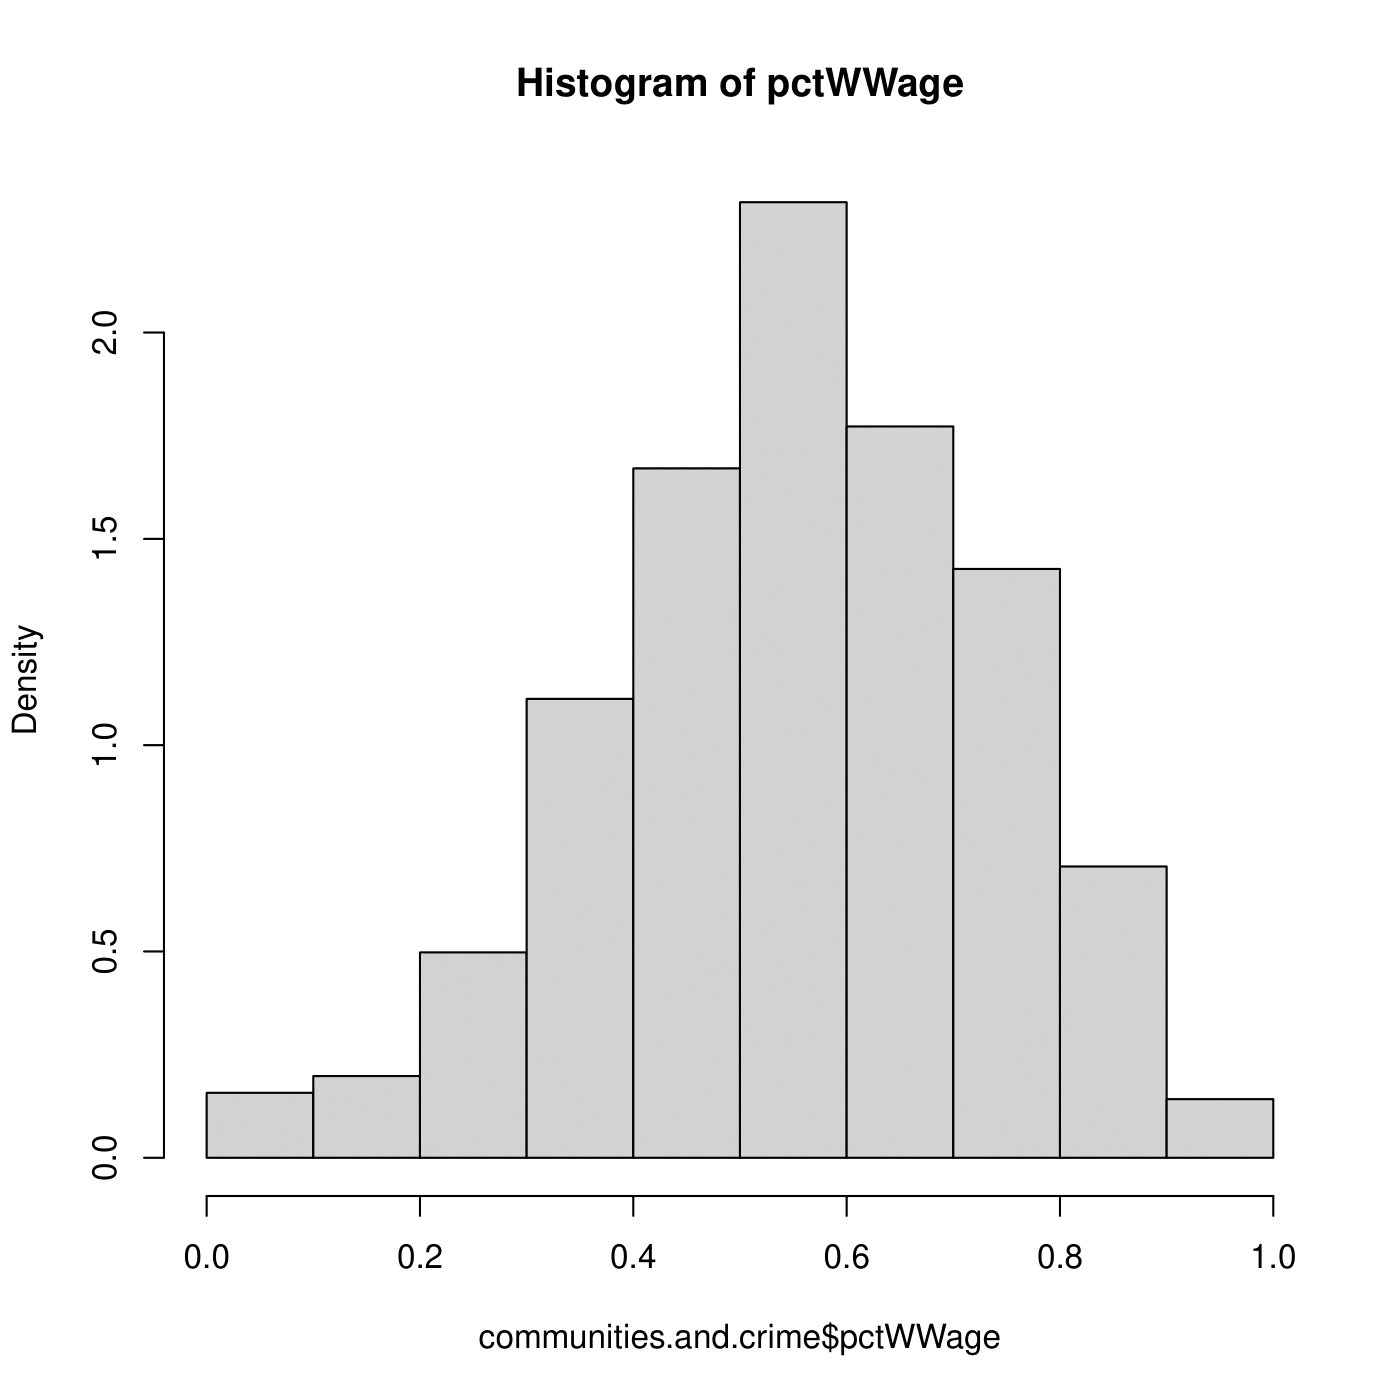
\includegraphics[width=0.45\textwidth]{normal/pctWWage_hist}
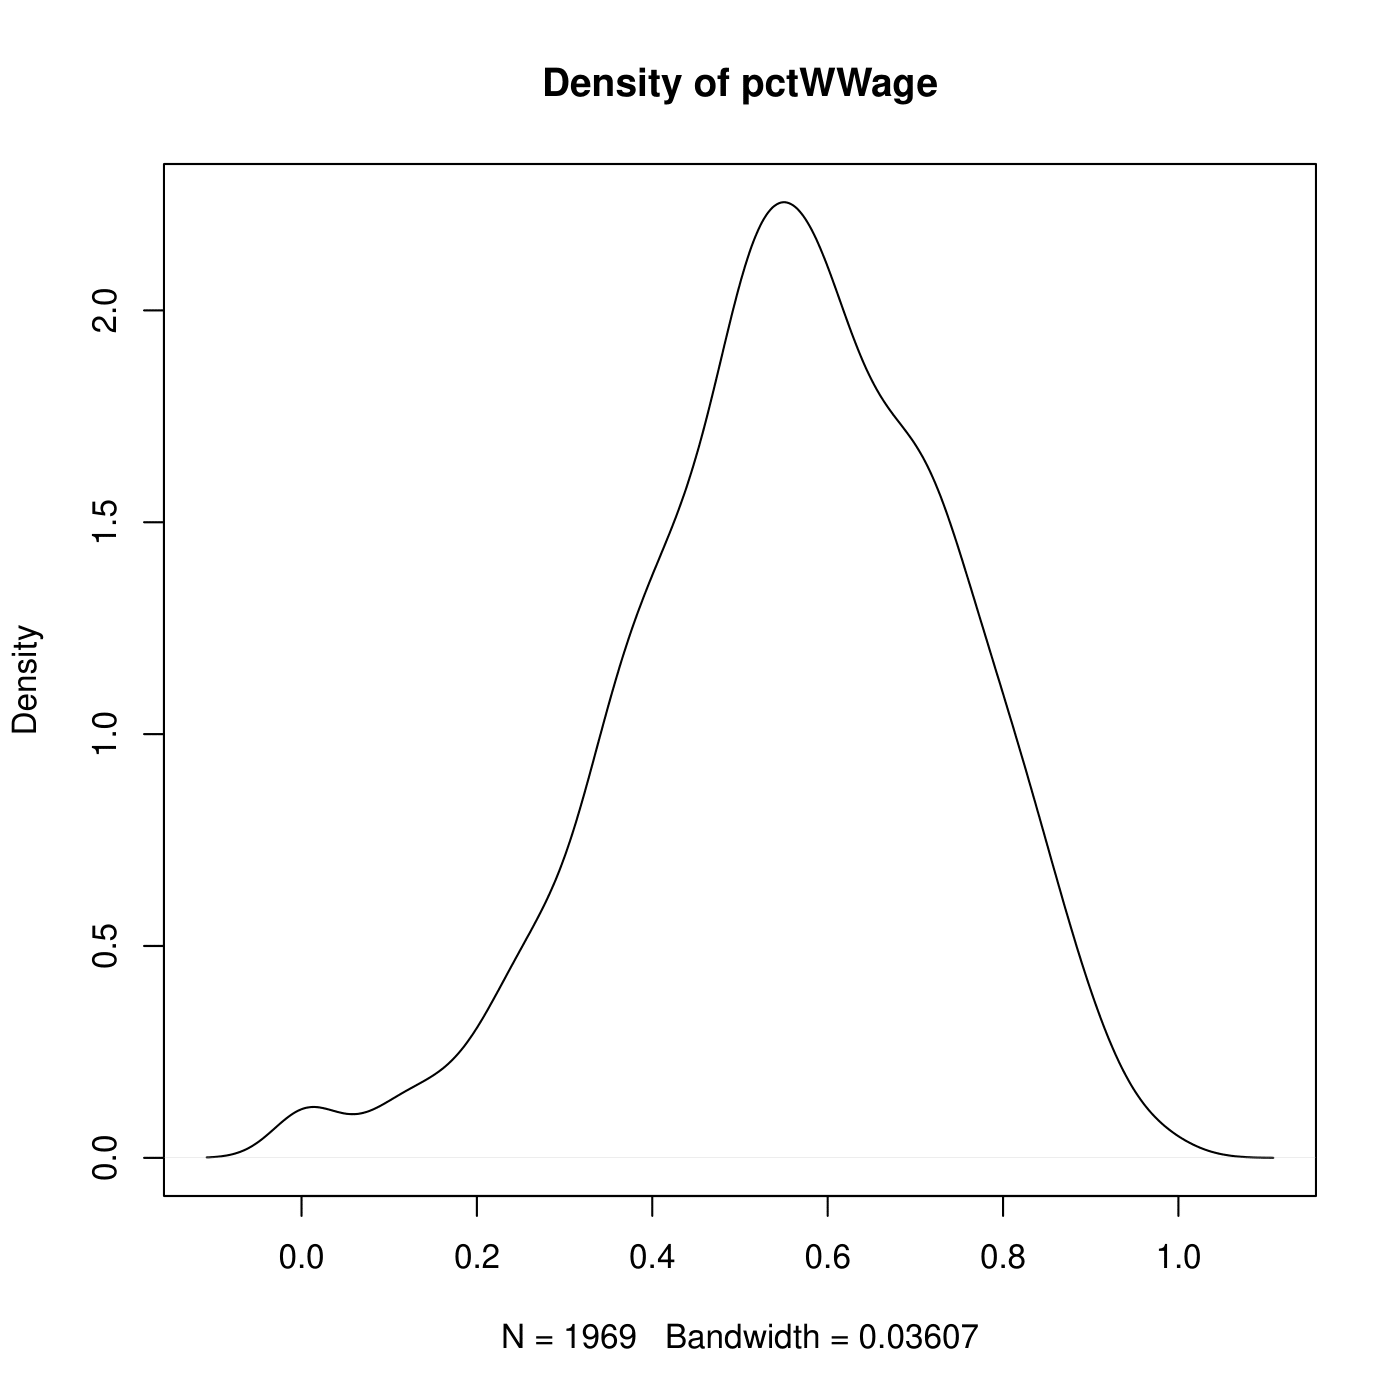
\includegraphics[width=0.45\textwidth]{normal/pctWWage_density}
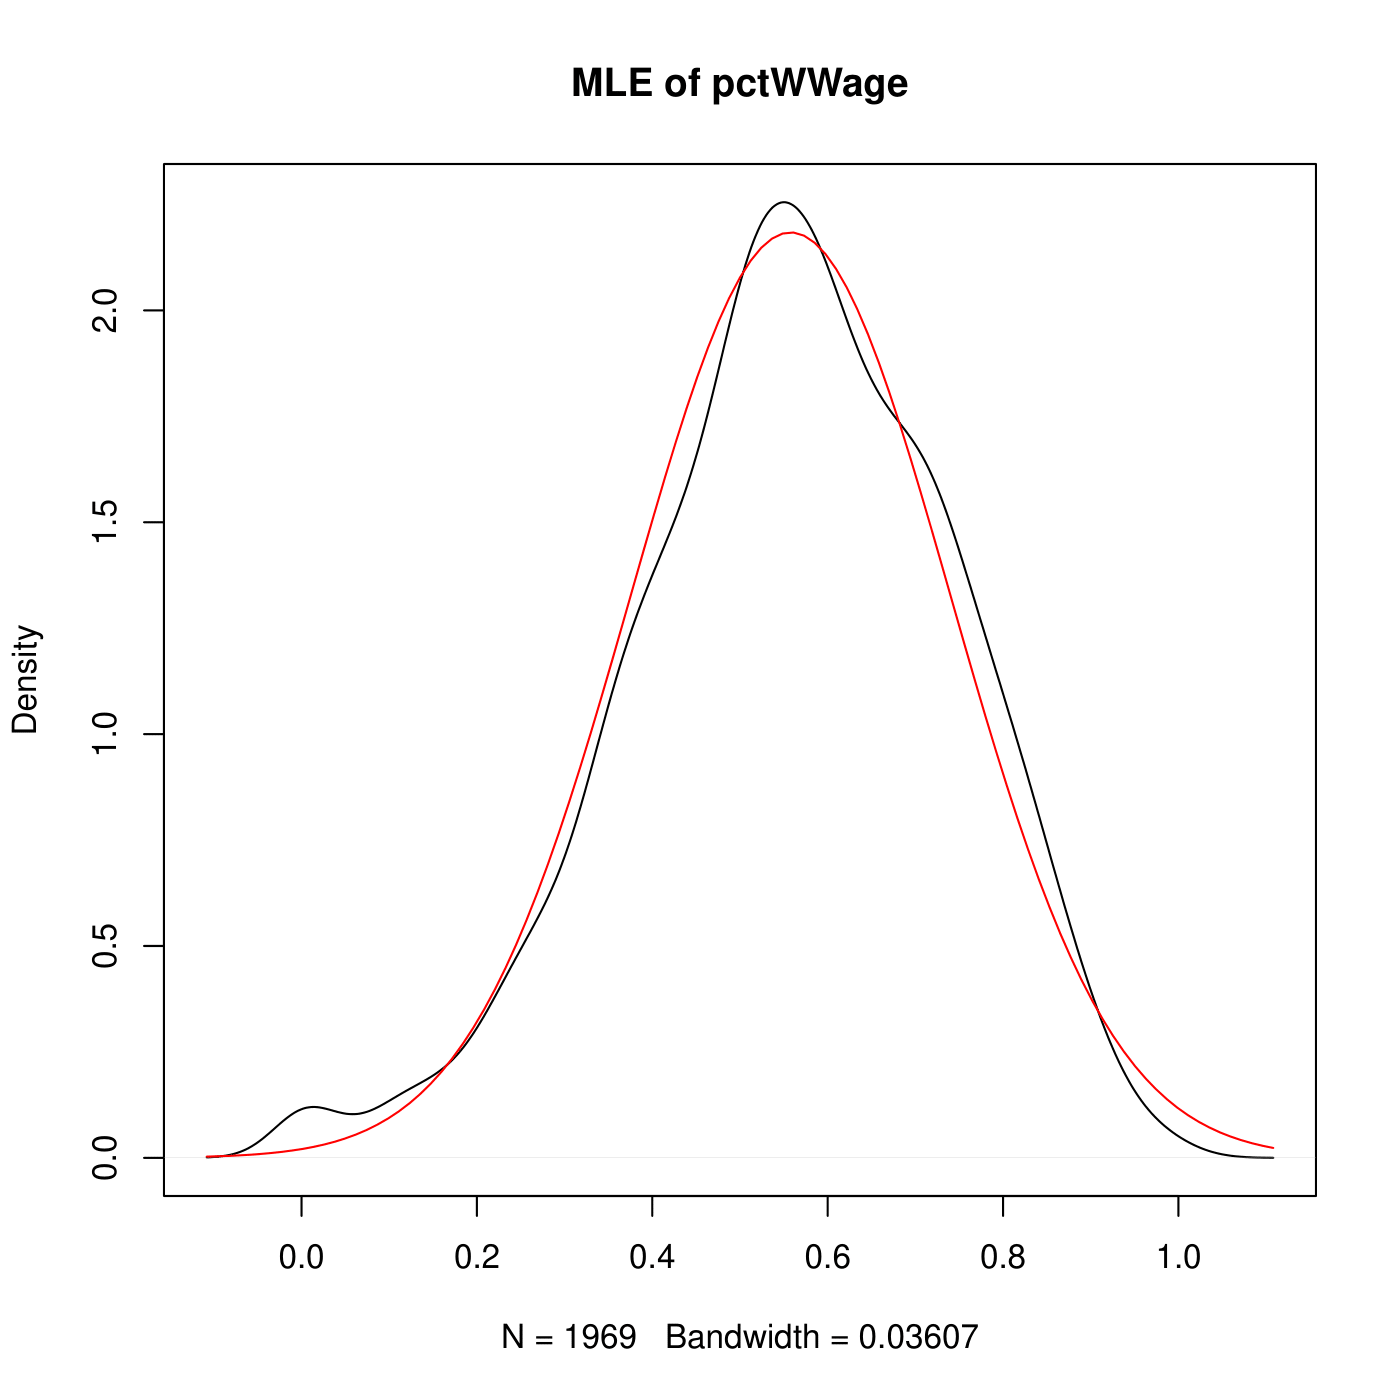
\includegraphics[width=0.45\textwidth]{normal/pctWWage_mle}
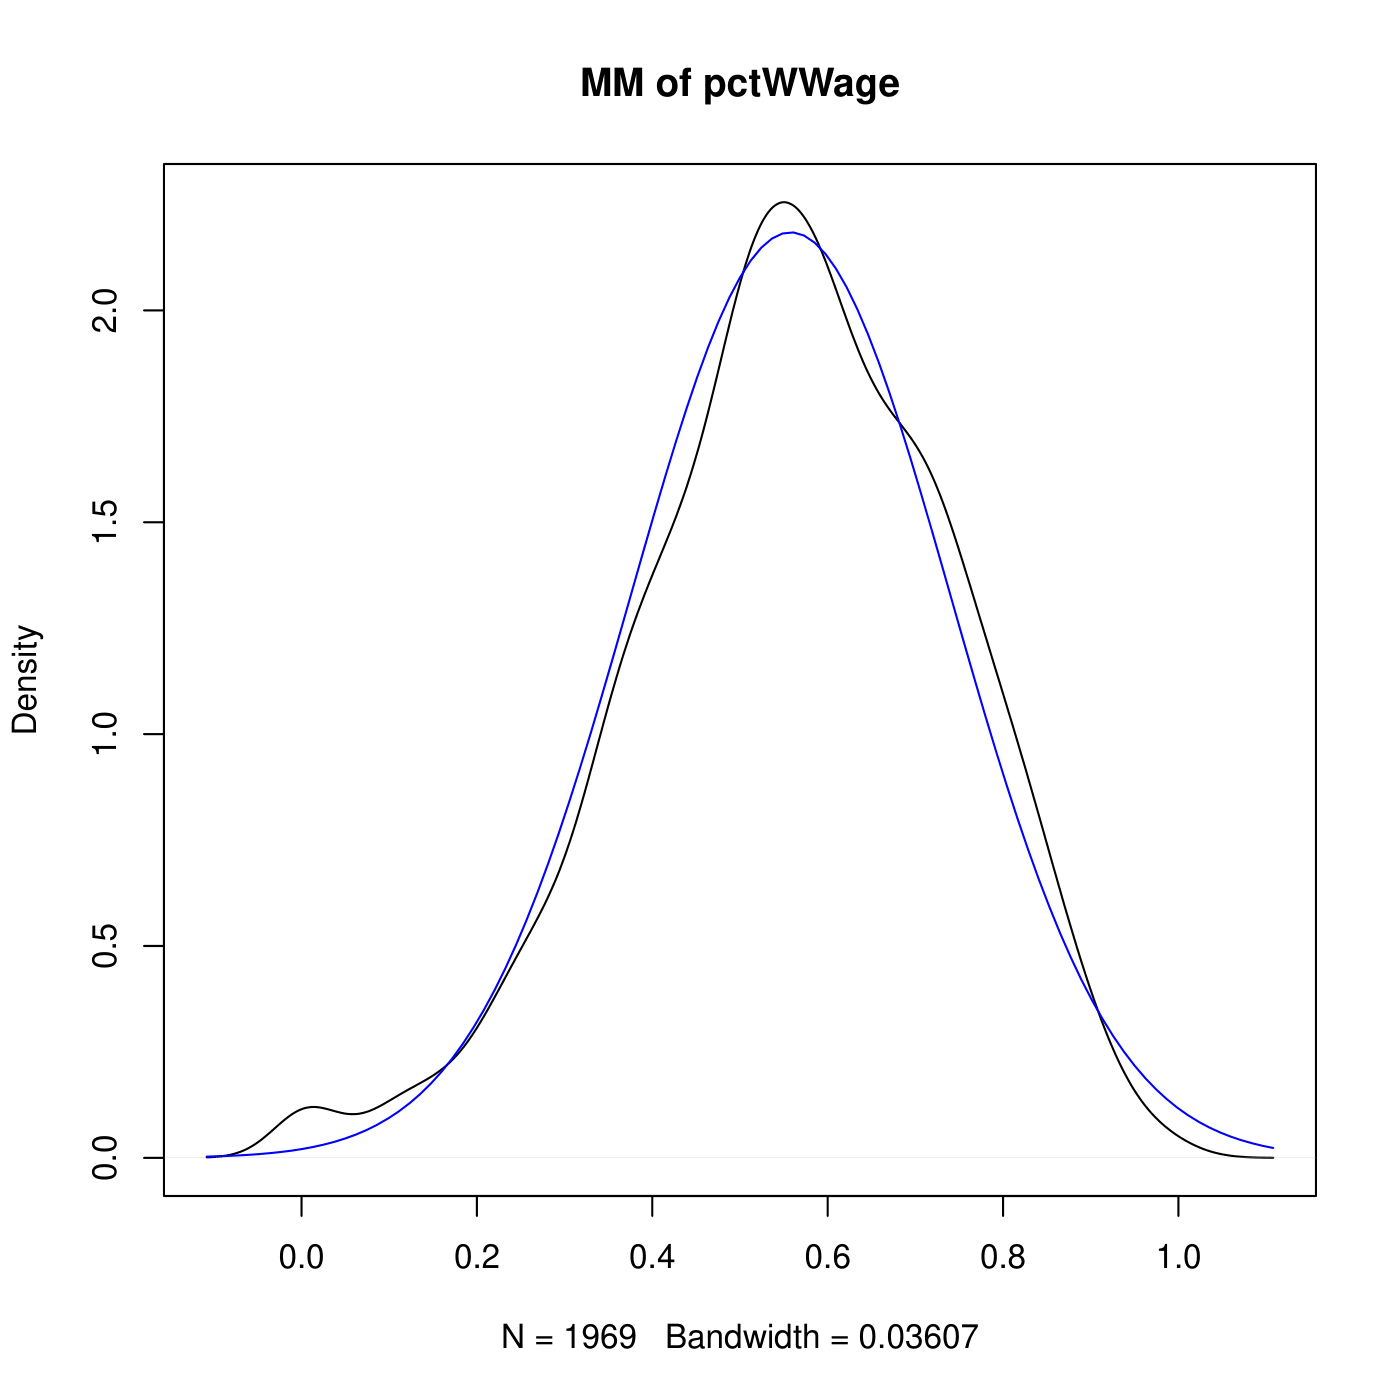
\includegraphics[width=0.45\textwidth]{normal/pctWWage_mm}
\end{center}


\maketitle
\chapter{The Exponential Family}
\section{Communities and Crime: PctLargHouseFam}

For the exponential family of continuous distributions, we observed that the variable \textbf{PctLargHouseFam} was a suitable approximation. 
According to the UCI Machine Learning Repository, \textbf{PctLargHouseFam} is described as the percentage of family households with six or more family members. 

\begin{center}
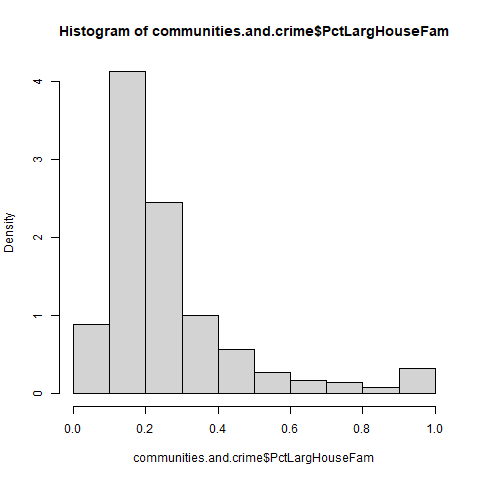
\includegraphics[width=0.45\textwidth]{exponential/PctLargHouseFam_hist}
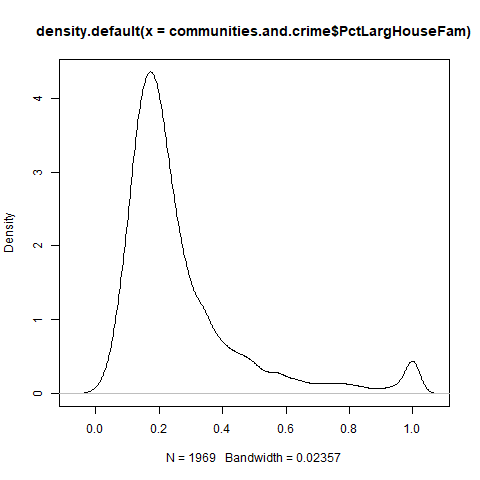
\includegraphics[width=0.45\textwidth]{exponential/PctLargHouseFam_density}
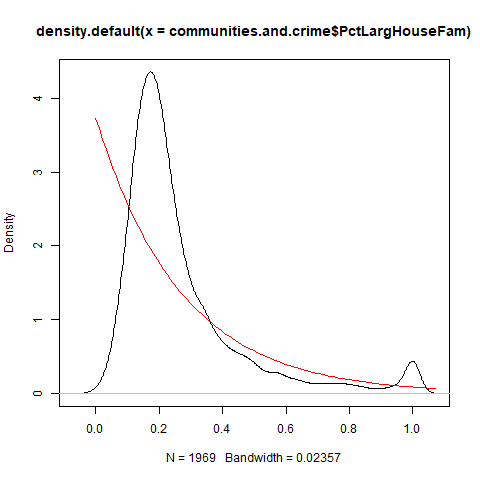
\includegraphics[width=0.45\textwidth]{exponential/PctLargHouseFam_mle}
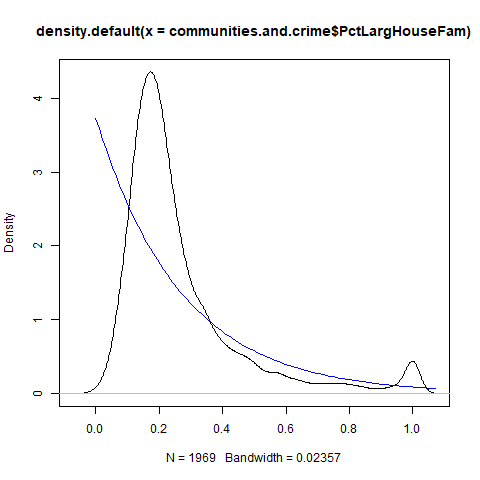
\includegraphics[width=0.45\textwidth]{exponential/PctLargHouseFam_mm}
\end{center}


\maketitle
\chapter{The Gamma Family}
\section{Communities and Crime: PctNotHsGrad}

We observed that the variable \textbf{PctNotHsGrad} of the Communities and Crime dataset seemed well-approximated by the gamma family of continuous distributions.
According to the UCI Machine Learning Repository, \textbf{PctNotHsGrad} is described as the percentage of people 25 and over that are not high school graduates.

\begin{center}
\includegraphics[width=0.45\textwidth]{gamma/PctNotHsGrad_hist}
\includegraphics[width=0.45\textwidth]{gamma/PctNotHsGrad_density}
\includegraphics[width=0.45\textwidth]{gamma/PctNotHsGrad_mle}
\includegraphics[width=0.45\textwidth]{gamma/PctNotHsGrad_mm}
\end{center}


\maketitle
\chapter{The Beta Family}
\section{Communities and Crime: PctNotSpeakEnglWell}

For the beta family of continuous distributions, we observed that the variable \textbf{PctNotSpeakEnglWell} was a suitable approximation. 
According to the UCI Machine Learning Repository, \textbf{PctNotSpeakEnglWell} is described as the percentage of people who do not speak English well. 

\begin{center}
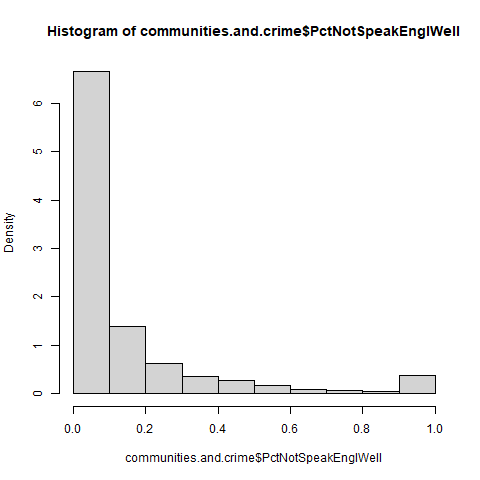
\includegraphics[width=0.45\textwidth]{beta/PctNotSpeakEnglWell_hist}
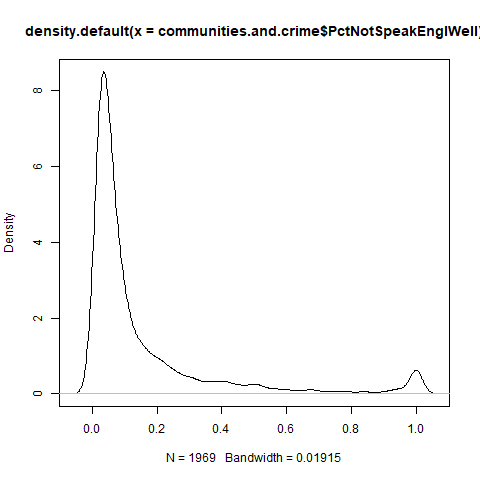
\includegraphics[width=0.45\textwidth]{beta/PctNotSpeakEnglWell_density}
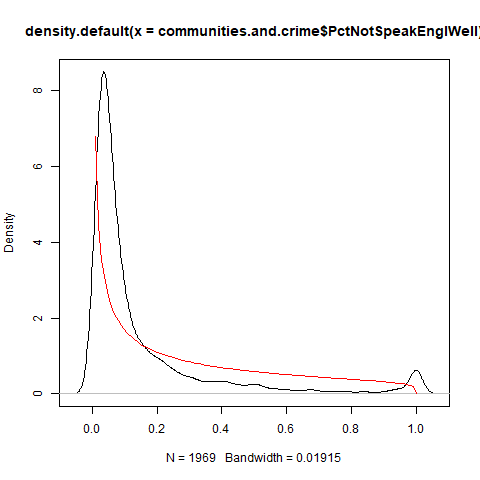
\includegraphics[width=0.45\textwidth]{beta/PctNotSpeakEnglWell_mle}
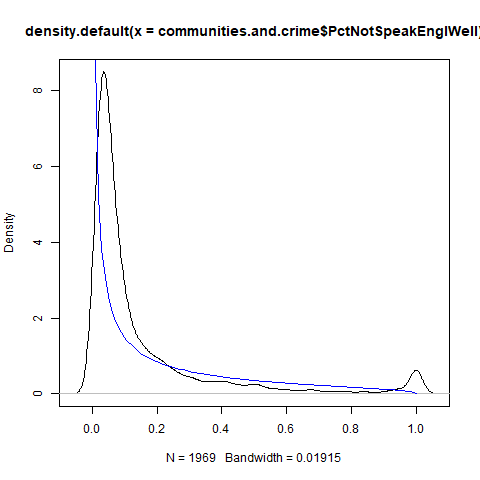
\includegraphics[width=0.45\textwidth]{beta/PctNotSpeakEnglWell_mm}
\end{center}

\end{document}